\documentclass[10pt,leqno]{article}

\usepackage[%
  tmargin=1.2in,bmargin=1.2in,%
  lmargin=1.8in,rmargin=1.8in,%
]{geometry}
\usepackage{fancyhdr}
\usepackage{titlesec}
\usepackage{appendix}
\usepackage{microtype}
\usepackage[hyphens]{url}
\usepackage{enumitem}
\usepackage{xspace}
\usepackage{etoolbox}
\usepackage{ifthen}
\usepackage{tikz}
\usepackage{tikz-cd}

\usepackage{amsmath}
\definecolor{darkred}{rgb}{0.5,0.0,0.0}
\usepackage[%
  colorlinks,%
  linkcolor=darkred,%
  citecolor=darkred,%
  urlcolor=darkred,%
]{hyperref}
\usepackage{amsthm,amssymb}
% \usepackage[lining,semibold]{libertine}
% \usepackage{textcomp,stmaryrd}
% \usepackage[libertine,cmintegrals,bigdelims]{newtxmath}
% \useosf
% \usepackage[%
%   cal=boondox, calscaled=0.97,%
%   bb=boondox, bbscaled=0.98,%
% ]{mathalfa}
\usepackage{cleveref}

\frenchspacing
\urlstyle{rm}

\AtBeginDocument{%
  \setlength{\abovedisplayskip}{1.5ex plus 0.3ex minus 0.3ex}%
  \setlength{\abovedisplayshortskip}{1.0ex plus 0.3ex minus 0.3ex}%
  \setlength{\belowdisplayskip}{1.5ex plus 0.3ex minus 0.3ex}%
  \setlength{\belowdisplayshortskip}{1.0ex plus 0.3ex minus 0.3ex}%
}

\let\theoldbibliography\thebibliography
\renewcommand{\thebibliography}[1]{%
  \theoldbibliography{#1}%
  \setlength{\parskip}{0ex}
  \setlength{\itemsep}{0.5ex plus 0.2ex minus 0.2ex}
  \small
}

\pagestyle{fancy}
\renewcommand{\headrulewidth}{0pt}
\renewcommand{\footrulewidth}{0pt}
\fancyhf{}
\fancyfoot[C]{\small\thepage}

\renewcommand{\title}[1]{\newcommand{\thetitle}{#1}}
\renewcommand{\author}[1]{\newcommand{\theauthor}{#1}}
\renewcommand{\date}[1]{\newcommand{\thedate}{#1}}

\renewcommand{\maketitle}{%
  \begin{center}
    {\bfseries\MakeUppercase{%
      \thetitle}}\\[2.5ex]
    {\footnotesize\MakeUppercase{%
      \theauthor}}\\[2.5ex]
    \ifthenelse{\equal{\thedate}{}}{}{%
      \small%
      \setlength{\tabcolsep}{0.2em}%
      \begin{tabular}{rl}
        original: & \thedate \\
        updated: & \today
      \end{tabular}
    }
  \end{center}
  \vspace{2.5ex}
  \thispagestyle{fancy}
}

%%%%%%%%%%%%%%%%%%%%%%%%%%%%%%%%%%%%%%%%%%%%%%%%%%%%%%%%%%%%%%%%%%%%%%

\cspreto{section}{\setcounter{equation}{0}}

\titleformat{\section}{\centering\scshape}{\thesection.}{0.4em}{}
\titlespacing{\section}{0pt}{*4}{*1}
\titleformat{\subsection}{\scshape}{\thesubsection.}{0.4em}{}
\titlespacing{\subsection}{0pt}{*2.5}{*1}

% Display format for equations
\newcommand{\crefeqfmt}[1]{
  \crefformat{#1}{(##2##1##3)}
  \Crefformat{#1}{(##2##1##3)}
  \crefrangeformat{#1}{(##3##1##4--##5##2##6)}
  \Crefrangeformat{#1}{(##3##1##4--##5##2##6)}
  \crefmultiformat{#1}{(##2##1##3}{, ##2##1##3)}{, ##2##1##3}{, ##2##1##3)}
  \Crefmultiformat{#1}{(##2##1##3}{, ##2##1##3)}{, ##2##1##3}{, ##2##1##3)}
  \crefrangemultiformat{#1}{(##3##1##4--##5##2##6}{, ##3##1##4--##5##2##6)}{, ##3##1##4--##5##2##6}{, ##3##1##4--##5##2##6)}
  \Crefrangemultiformat{#1}{(##3##1##4--##5##2##6}{, ##3##1##4--##5##2##6)}{, ##3##1##4--##5##2##6}{, ##3##1##4--##5##2##6)}
}
% Display format for sections
\newcommand{\crefsecfmt}[1]{%
  \crefformat{#1}{\S##2##1##3}
  \Crefformat{#1}{\S##2##1##3}
  \crefrangeformat{#1}{\S\S##3##1##4--##5##2##6}
  \Crefrangeformat{#1}{\S\S##3##1##4--##5##2##6}
  \crefmultiformat{#1}{\S\S##2##1##3}{ and~##2##1##3}{, ##2##1##3}{ and~##2##1##3}
  \Crefmultiformat{#1}{\S\S##2##1##3}{ and~##2##1##3}{, ##2##1##3}{ and~##2##1##3}
  \crefrangemultiformat{#1}{\S\S##3##1##4--##5##2##6}{ and~##3##1##4--##5##2##6}{, ##3##1##4--##5##2##6}{ and~##3##1##4--##5##2##6}
  \Crefrangemultiformat{#1}{\S\S##3##1##4--##5##2##6}{ and~##3##1##4--##5##2##6}{, ##3##1##4--##5##2##6}{ and~##3##1##4--##5##2##6}
}
\crefeqfmt{equation}
\crefeqfmt{enumi}
\crefeqfmt{enumii}
\crefsecfmt{section}
\crefsecfmt{subsection}
\crefsecfmt{appendix}
\crefname{part}{Part}{Parts}
\crefname{chapter}{Chapter}{Chapters}
\crefname{figure}{Figure}{Figures}

\makeatletter

\newcommand{\thmnumfont}{\bfseries}
\newcommand{\thmheadfont}{\bfseries}
\newcommand{\thmnotefont}{\bfseries}
\newcommand{\thmhorizspace}{0.4em}

\def\swappedhead#1#2#3{%
  \thmnumber{\@upn{{\thmnumfont#2}}\@ifnotempty{#1}{.\hspace{0.25em}}}%
  \thmheadfont\thmname{#1}%
  \@ifnotempty{#3}{\ \thmnote{\thmnotefont(#3)}}%
}
\swapnumbers

\newtheoremstyle{block}%
  {2.0ex plus 0.2ex minus 0.1ex}% Space above
  {2.0ex plus 0.2ex minus 0.1ex}% Space below
  {} % Body font
  {} % Indent amount
  {\thmheadfont} % Theorem head font
  {.} % Punctuation after theorem head
  {\thmhorizspace} % Space after theorem head
  {} % Theorem head spec (can be left empty, meaning ‘normal’)

\renewenvironment{proof}[1][Proof]{\par
  \pushQED{\qed}%
  \normalfont%
  \topsep1ex plus 0.2ex minus 0.1ex\relax%
  \labelsep \thmhorizspace\relax%
  \trivlist
  \item[\hskip\labelsep\thmheadfont
    #1\@addpunct{.}]\ignorespaces
}{%
  \popQED\endtrivlist\@endpefalse%
}

\makeatother

\theoremstyle{block}

\newcommand{\defthm}[2]{%
  \newtheorem{#1}[equation]{#2}%
  \crefeqfmt{#1}%
  \newtheorem*{#1*}{#2}%
}

\defthm{algorithm}{Algorithm}
\defthm{conjecture}{Conjecture}
\defthm{construction}{Construction}
\defthm{convention}{Convention}
\defthm{corollary}{Corollary}
\defthm{definition}{Definition}
\defthm{definitions}{Definitions}
\defthm{example}{Example}
\defthm{examples}{Examples}
\defthm{exercise}{Exercise}
\defthm{fact}{Fact}
\defthm{intuition}{Intuition}
\defthm{lemma}{Lemma}
\defthm{notation}{Notation}
\defthm{nothing}{}
\defthm{proposition}{Proposition}
\defthm{question}{Question}
\defthm{remark}{Remark}
\defthm{remarks}{Remarks}
\defthm{situtation}{Situation}
\defthm{theorem}{Theorem}

\setlist{%
  leftmargin=2.5em, parsep=0ex, listparindent=\parindent,
  itemsep=1.0ex, topsep=1.0ex,%
}

\setlist[enumerate, 1]{%
  label=(\alph*),%
  ref=\alph*,%
  widest=d,%
}
\setlist[enumerate, 2]{%
  label=(\roman*),%
  ref=\theenumi.\roman*,%
}
\setlist[itemize, 1]{%
  label=$\vcenter{\hbox{\footnotesize$\bullet$}}$,%
}
\setlist[itemize, 2]{label=--}

%%%%%%%%%%%%%%%%%%%%%%%%%%%%%%%%%%%%%%%%%%%%%%%%%%%%%%%%%%%%%%%%%%%%%%

\makeatletter

\let\ea\expandafter

\newcount\foreachcount

\def\foreachletter#1#2#3{\foreachcount=#1
  \ea\loop\ea\ea\ea#3\@alph\foreachcount
  \advance\foreachcount by 1
  \ifnum\foreachcount<#2\repeat}

\def\foreachLetter#1#2#3{\foreachcount=#1
  \ea\loop\ea\ea\ea#3\@Alph\foreachcount
  \advance\foreachcount by 1
  \ifnum\foreachcount<#2\repeat}

% Roman: \rA is \mathrm{A}
\def\definerm#1{%
  \ea\gdef\csname r#1\endcsname{\ensuremath{\mathrm{#1}}\xspace}}
\foreachLetter{1}{27}{\definerm}
\foreachletter{1}{27}{\definerm}
% Script: \sA is \mathscr{A}
\def\definescr#1{%
  \ea\gdef\csname s#1\endcsname{\ensuremath{\mathscr{#1}}\xspace}}
\foreachLetter{1}{27}{\definescr}
% Calligraphic: \cA is \mathcal{A}
\def\definecal#1{%
  \ea\gdef\csname c#1\endcsname{\ensuremath{\mathcal{#1}}\xspace}}
\foreachLetter{1}{27}{\definecal}
% Bold: \bA is \mathbf{A}
\def\definebold#1{%
  \ea\gdef\csname b#1\endcsname{\ensuremath{\mathbf{#1}}\xspace}}
\foreachLetter{1}{27}{\definebold}
% Blackboard Bold: \lA is \mathbb{A}
\def\definebb#1{%
  \ea\gdef\csname l#1\endcsname{\ensuremath{\mathbb{#1}}\xspace}}
\foreachLetter{1}{27}{\definebb}
% Fraktur: \ka is \mathfrak{a}, \kA is \mathfrak{A}
\def\definefrak#1{%
  \ea\gdef\csname k#1\endcsname{\ensuremath{\mathfrak{#1}}\xspace}}
\foreachletter{1}{27}{\definefrak}
\foreachLetter{1}{27}{\definefrak}
% Sans serif: \iA \is \mathsf{A}
\def\definesf#1{%
  \ea\gdef\csname i#1\endcsname{\ensuremath{\mathsf{#1}}\xspace}}
\foreachletter{1}{6}{\definesf}
\foreachletter{7}{14}{\definesf}
\foreachletter{15}{27}{\definesf}
\foreachLetter{1}{27}{\definesf}
% Bar: \Abar is \overline{A}, \abar is \overline{a}
\def\definebar#1{%
  \ea\gdef\csname #1bar\endcsname{\ensuremath{\overline{#1}}\xspace}}
\foreachLetter{1}{27}{\definebar}
\foreachletter{1}{8}{\definebar} % \hbar is something else!
\foreachletter{9}{15}{\definebar} % \obar is something else!
\foreachletter{16}{27}{\definebar}
% Tilde: \Atil is \widetilde{A}, \atil is \widetilde{a}
\def\definetil#1{%
  \ea\gdef\csname #1til\endcsname{\ensuremath{\widetilde{#1}}\xspace}}
\foreachLetter{1}{27}{\definetil}
\foreachletter{1}{27}{\definetil}
% Hats: \Ahat is \widehat{A}, \ahat is \widehat{a}
\def\definehat#1{%
  \ea\gdef\csname #1hat\endcsname{\ensuremath{\widehat{#1}}\xspace}}
\foreachLetter{1}{27}{\definehat}
\foreachletter{1}{27}{\definehat}
% Checks: \Achk is \widecheck{A}, \achk is \widecheck{a}
\def\definechk#1{%
  \ea\gdef\csname #1chk\endcsname{\ensuremath{\widecheck{#1}}\xspace}}
\foreachLetter{1}{27}{\definechk}
\foreachletter{1}{27}{\definechk}
% Underline: \Aund is \underline{A}, \aund is \underline{a}
\def\defineul#1{%
  \ea\gdef\csname #1und\endcsname{\ensuremath{\underline{#1}}\xspace}}
\foreachLetter{1}{27}{\defineul}
\foreachletter{1}{27}{\defineul}

\makeatother

%%%%%%%%%%%%%%%%%%%%%%%%%%%%%%%%%%%%%%%%%%%%%%%%%%%%%%%%%%%%%%%%%%%%%%

\usetikzlibrary{calc,decorations.pathmorphing,shapes,arrows}
\tikzcdset{
  arrow style=tikz,
  diagrams={>={stealth}},
}

\newcommand{\arrlen}{1em}
\renewcommand{\to}{\mathrel{\tikz[baseline]%
    \draw[>=stealth,->](0,0.5ex)--(\arrlen,0.5ex);}}
\newcommand{\from}{\mathrel{\tikz[baseline]%
    \draw[>=stealth,<-](0,0.5ex)--(\arrlen,0.5ex);}}
\renewcommand{\mapsto}{\mathrel{\tikz[baseline]%
    \draw[>=stealth,|->](0,0.5ex)--(\arrlen,0.5ex);}}
\newcommand{\inj}{\mathrel{\tikz[baseline]%
    \draw[>=stealth,right hook->](0,0.5ex)--(\arrlen,0.5ex);}}
\newcommand{\surj}{\mathrel{\tikz[baseline]%
    \draw[>=stealth,->>](0,0.5ex)--(\arrlen,0.5ex);}}
\newcommand{\fromto}{\mathrel{%
  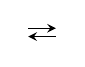
\begin{tikzpicture}[baseline]%
    \draw[>=stealth,<-](0,0.15ex)--(\arrlen,0.15ex);%
    \draw[>=stealth,->](0,0.85ex)--(\arrlen,0.85ex);%
  \end{tikzpicture}}}
\newcommand{\doubto}{\mathrel{%
  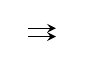
\begin{tikzpicture}[baseline]%
    \draw[>=stealth,->](0,0.15ex)--(\arrlen,0.15ex);%
    \draw[>=stealth,->](0,0.85ex)--(\arrlen,0.85ex);%
  \end{tikzpicture}}}
\newcommand{\lblto}[1]{\mathrel{%
    \begin{tikzpicture}[baseline= {( $ (current bounding box.south) + (0,-0.5ex) $ )}]
      \node[inner sep=.4ex] (a) {\,$\scriptstyle #1$\,};
      \draw[>=stealth,->] (a.south west) -- (a.south east);
    \end{tikzpicture}}}
\newcommand{\isoto}{\lblto{\sim}}

\newcommand{\simpl}[3]{
  \begin{tikzcd}[ampersand replacement=\&, column sep=small]
    #1 \&
    #2 \ar[l, shift right=0.35ex]
       \ar[l, shift left=0.35ex] \&
    #3 \ar[l, shift right=0.70ex]
       \ar[l, shift left=0.70ex]
       \ar[l] \&
    \cdots \ar[l, shift right=0.35ex]
           \ar[l, shift left=0.35ex]
           \ar[l, shift right=1.05ex]
           \ar[l, shift left=1.05ex]
  \end{tikzcd}
}
\newcommand{\cosimpl}[3]{
  \begin{tikzcd}[ampersand replacement=\&, column sep=small]
    #1 \ar[r, shift right=0.35ex]
       \ar[r, shift left=0.35ex] \&
    #2 \ar[r, shift right=0.70ex]
       \ar[r, shift left=0.70ex]
       \ar[r] \&
    #3 \ar[r, shift right=0.35ex]
       \ar[r, shift left=0.35ex]
       \ar[r, shift right=1.05ex]
       \ar[r, shift left=1.05ex] \&
    \cdots
  \end{tikzcd}
}

\newcommand{\tto}{\mathrel{\tikz[baseline]%
    \draw[>=stealth,->,double, double distance = 0.3ex](0,0.5ex)--(\arrlen,0.5ex);}}
\newcommand{\doubfrom}{\mathrel{%
  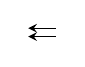
\begin{tikzpicture}[baseline]%
    \draw[>=stealth,<-](0,0.15ex)--(\arrlen,0.15ex);%
    \draw[>=stealth,<-](0,0.85ex)--(\arrlen,0.85ex);%
  \end{tikzpicture}}}
\newcommand{\tripfrom}{\mathrel{%
  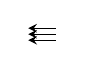
\begin{tikzpicture}[baseline]%
    \draw[>=stealth,<-](0,0.00ex)--(\arrlen,0.00ex);%
    \draw[>=stealth,<-](0,0.50ex)--(\arrlen,0.50ex);%
    \draw[>=stealth,<-](0,1.00ex)--(\arrlen,1.00ex);%
  \end{tikzpicture}}}


\renewcommand{\l}{\left}
\renewcommand{\r}{\right}
\newcommand{\f}{\frac}
\renewcommand{\o}{\overline}
\renewcommand{\u}{\underline}
\newcommand{\til}{\widetilde}
\renewcommand{\hat}{\widehat}
\newcommand{\del}{\partial}
\newcommand{\dash}{\text{-}}
\renewcommand{\c}{\colon}
\newcommand{\lc}{\,:\!}
\newcommand{\ce}{\coloneq}%{\mathrel{:=}}
\newcommand{\ec}{\eqcolon}%{\mathrel{=:}}
\newcommand{\iso}{\simeq}
\newcommand{\dual}{\vee}
\newcommand{\ldb}{\llbracket}
\newcommand{\rdb}{\rrbracket}

\newcommand{\Obj}{\operatorname{Obj}}
\newcommand{\Hom}{\operatorname{Hom}}
\newcommand{\Map}{\operatorname{Map}}
\newcommand{\Fun}{\operatorname{Fun}}
\newcommand{\Aut}{\operatorname{Aut}}
\newcommand{\Iso}{\operatorname{Iso}}
\renewcommand{\id}{\mathrm{id}}
\renewcommand{\im}{\operatorname{im}}
\newcommand{\op}{\mathrm{op}}
\newcommand{\univ}{\mathrm{univ}}
\newcommand{\colim}{\operatorname*{colim}}
\newcommand{\dlim}{\displaystyle\lim}
\newcommand{\dcolim}{\displaystyle\colim}
\newcommand{\Spec}{\operatorname{Spec}}
\newcommand{\Spf}{\operatorname{Spf}}

%%%%%%%%%%%%%%%%%%%%%%%%%%%%%%%%%%%%%%%%%%%%%%%%%%%%%%%%%%%%%%%%%%%%%%


\title{The Dennis trace (and why you might care)}
\author{Arpon Raksit}
\date{November 11, 2016}

\begin{document}
\maketitle

\numberwithin{block}{section}
\addtocounter{section}{-1}

\newcommand{\A}{\operatorname{A}}
\newcommand{\ab}{\mathrm{ab}}
\newcommand{\Conc}{\operatorname{Conc}}
\newcommand{\GL}{\operatorname{GL}}
\newcommand{\hCob}{\operatorname{Cob_h}}
\newcommand{\HH}{\operatorname{HH}}
\newcommand{\Homeo}{\operatorname{Homeo}}
\newcommand{\K}{\operatorname{K}}
\newcommand{\Wh}{\operatorname{Wh}}

%%%%%%%%%%%%%%%%%%%%%%%%%%%%%%%%%%%%%%%%%%%%%%%%%%%%%%%%%%%%%%%%%%%%%%

\section{Introduction}
\label{intro}

I have two goals in this talk.\footnote{These are notes for a talk given in the student topology seminar at Stanford in fall 2016.}

The first is to reveal why algebraic K-theory and Hochschild/cyclic homology belong in the same seminar, by constructing the \emph{Dennis trace map}
\[
\K_*(R) \to \HH_*(R)
\]
and explaining some of its features.

The second is to persuade you (i.e. someone interested in topology) to care about higher algebraic K-theory and the Dennis trace map, by outlining a story, extending the ideas of the s-cobordism theorem discussed earlier in the seminar, whose moral is that higher algebraic K-theory really knows a great deal about manifold topology.

We'll see how it goes.

%%%%%%%%%%%%%%%%%%%%%%%%%%%%%%%%%%%%%%%%%%%%%%%%%%%%%%%%%%%%%%%%%%%%%%

\section{Constructing the Dennis trace}
\label{dennis}

\todo[inline]{write the main section of the talk...}

%%%%%%%%%%%%%%%%%%%%%%%%%%%%%%%%%%%%%%%%%%%%%%%%%%%%%%%%%%%%%%%%%%%%%%

\section{Algebraic K-theory and manifold topology}
\label{manifolds}

I now want to give some topological motivation for higher algebraic K-theory, and explain why the Dennis trace is useful in the context of this motivation. This is going to be an outline of a (hopefully compelling) story; I don't know any of the details yet, so they certainly won't be appearing here. \todo{Mention references (Lurie, Rognes, ...)}

\begin{convention}
  \label{manfiolds-topological}
  Throughout this discussion, let us take ``manifold'' to mean \emph{topological} manifold. (Similar stories can be told for the PL and smooth cases.)
\end{convention}

\begin{nothing}
  \label{manifolds-goal}
  Let's set ourselves the goal of classifying all closed manifolds, say of a fixed dimension $d$. What exactly do we mean by this though?

  To a zeroth order, classification would mean some kind of description of the set of homeomorphism classes of manifolds. This already sounds incredibly ambitious, but there is more information in the world of manifolds than this set. Namely, we'd also like to classify the homeomorphisms $\Homeo(M,N)$ between any two manifolds $M$, $N$, or equivalently the self-homeomorphisms $\Homeo(M,M)$ for any manifold $M$.

  But we have to decide to what extent we want to describe $\Homeo(M,M)$, i.e. we have to decide what kind of object it is. It's certainly a group, but as usual there is a natural mapping space topology on it, making it is a topological group. In this topology, it's something infinite-dimensional and hence quite frightening maybe, but the topology does contain information we might be interested in; e.g. a path in $\Homeo(M,M)$ corresponds to an isotopy of homeomorphisms. To achieve some kind of balance, let's say that we'd just like to describe the \emph{homotopy type} of $\Homeo(M,M)$; this will hopefully mitigate the forbidding infinite-dimensionality while retaining information about paths/isotopies and the like.

  Motivated by this discussion, we define the following moduli space.

  \begin{subdefinition}
    \label{manifolds-goal-moduli}
    We define the \emph{moduli space of closed $d$-dimensional manifolds} to be the homotopy type
    \[
      \sM \ce \coprod_{[M]} \rB\Homeo(M,M),
    \]
    where $[M]$ runs over the set of homeomorphism classes of closed $d$-dimensional manifolds $M$, and $\rB$ denotes the classifying space.
  \end{subdefinition}

  Our task can now be formulated as: describe the moduli space $\sM$ (as a homotopy type). To see why this is what we wanted, observe that:
  \begin{itemize}
  \item The set of connected components $\pi_0(\sM)$ is precisely the set of homeomorphism classes $[M]$ of closed $d$-dimensional manifolds $M$.
  \item For each point $M \in \sM$ (meaning any point in the connected component indexed by $[M]$), the homotopy type of the based loop space $\Omega_M\sM$ is precisely the space of self-homeomorphisms $\Homeo(M,M)$. More generally, for two points $M,N \in \sM$, the homotopy type of the path space $\sP_{M,N}\sM$ is the space $\Homeo(M,N)$.
  \end{itemize}

  \begin{subremark}
    \label{manifolds-goal-bundle}
    We should note that this moduli space $\sM$, like all moduli spaces, itself serves as a kind of classifying space. Namely, for nice topological spaces $B$, the set of homotopy classes of maps $B \to \sM$ is in natural bijection with the set of isomorphism classes of fiber bundles $E \to B$ whose fibers are closed $d$-dimensional manifolds.
  \end{subremark}
\end{nothing}

\begin{nothing}
  \label{manifolds-simplify}
  In \cref{manifolds-goal} we formulated our goal: classify closed $d$-dimensional manifolds by describing the moduli space of these, $\sM$. As mentioned above, this is quite a daunting problem, so we employ the usual strategy: first solve a simpler problem, and then try to bootstrap to a solution of the original problem.

  Here we will simplify our problem by relaxing the notion of equivalence between manifolds from homeomorphism to h-cobordism. Let's recall the definitions.

  \begin{subdefinition}
    \label{manifolds-simplify-cobordism}
    Let $M$ and $N$ be closed $d$-dimensional manifolds. A \emph{cobordism from $M$ to $N$} is a $(d+1)$-dimensional manifold $W$ equipped with a homeomorphism $M \amalg N \isoto \del W$. We say a cobordism is an \emph{h-cobordism} if the associated inclusion maps $M \inj W$ and $N \inj W$ are homotopy equivalences.
  \end{subdefinition}

  \begin{subexample}
    \label{manifolds-simplify-trivial-cobordism}
    Suppose given two closed manifolds $M,N$ and a homeomorphism $\phi \c N \isoto M$. Then the cylinder $M \times I$ equipped with the isomorphism
    \[
      \id_M \amalg \phi \c M \amalg N \isoto M \amalg M \iso \del(M \times I)
    \]
    is a cobordism of $M$ and $N$, and in fact it is evidently an h-cobordism.
  \end{subexample}

  We now want to construct a moduli space analogous to $\sM$ but with h-cobordism taking the role of homeomorphism.

  \begin{subdefinition}
    \label{manifolds-simplify-concordance}
    Let $M,N$ be two closed $d$-dimensional manifolds. Let
    \[
      (W_i,\phi_i \c M \amalg N \isoto \del W_i), \quad i \in \{1,2\}
    \]
    be two cobordisms from $M$ to $N$. A \emph{concordance} of cobordisms from $(W_1,\phi_1)$ to $(W_2,\phi_2)$ is a homeomorphism $\alpha \c W_1 \isoto W_2$ for which the diagram
    \[
      \begin{tikzcd}
        &
        M \amalg N \ar[dl, "\til\phi_1", swap] \ar[dr, "\til\phi_2"] &
        & \\
        W_1 \ar[rr, "\alpha"] &
        &
        W_2
      \end{tikzcd}
    \]
    commutes, where $\til\phi_i$ denotes the composite of $\phi_i$ with the inclusion of the boundary $\del W_i \inj W_i$.

    There is a natural mapping space topology on the collection of concordances from $(W_1,\phi_1)$ to $(W_2,\phi_2)$, and we will (abusively) denote the resulting topological space $\Conc(W_1,W_2)$. (Note that, as discussed in \cref{manifolds-goal} for spaces of homeomorphisms, we will only ever consider the \emph{homotopy types} of these spaces.)
  \end{subdefinition}

  \begin{subexample}
    \label{manifolds-simplify-isotopy}
    Let $M,N$ be two closed $d$-dimensional manifolds, and suppose given two homeomorphisms $\phi_1,\phi_2 \c N \isoto M$. From the construction of \cref{manifolds-simplify-trivial-cobordism} these determine two h-cobordisms from $M$ to $N$,
    \[
      (W_i,\psi_i) \ce (M \times I, \id_M \amalg \phi_i), \quad i \in \{1,2\}.
    \]
    Unravelling the definitions, one sees that a concordance $\alpha \c (W_1,\psi_1) \isoto (W_2,\psi_2)$ is precisely a \emph{pseudoisotopy} from $\id_M$ to the self-homeomorphism $\phi_2\phi_1^{-1} \c M \to M$. These are generalizations of isotopies from $\id_M$ to $\phi_2\phi_1^{-1}$, which are the pseudoisotopies that send $M \times \{t\}$ to $M \times \{t\}$ for each $t \in I$.

    Note that isotopies from $\id_M$ to $\phi_2\phi_1^{-1}$ are equivalent to isotopies from $\phi_1$ to $\phi_2$, so the latter also determine concordances from $W_1$ to $W_2$.
  \end{subexample}

  \begin{subdefinition}
    \label{manifolds-simplify-hcob-moduli}
    For $M,N$ two closed $d$-dimensional manifolds, define the \emph{space of h-cobordisms from $M$ to $N$} as
    \[
      \hCob(M,N) \ce \coprod_{[W]} \rB \Conc(W,W),
    \]
    where $[W]$ runs over the set of concordance classes of h-cobordisms $(W,\phi)$ from $M$ to $N$. From the fact that h-cobordisms can be composed and inverted, when $M=N$ we may think of $\hCob(M,M)$ as a topological group.\footnote{For the homotopical purists, what I really mean is that the homotopy type $\hCob(M,M)$ is a loop space.}

    Then, define the \emph{moduli space of closed $d$-dimensional manifolds up to h-cobordism} as the homotopy type
    \[
      \sH \ce \coprod_{\langle M \rangle} \rB \hCob(M,M),
    \]
    where $\langle M \rangle$ runs over the set of h-cobordism classes of closed $d$-dimensional manifolds $M$.
  \end{subdefinition}

  \begin{subremark}
    \label{manfiolds-simplify-moduli-unwrap}
    We understand the two homotopy types just defined analogously to $\sM$, as follows. For $\hCob(M,N)$:
    \begin{itemize}
    \item The set of connected components $\pi_0(\hCob(M,N))$ is the set of concordance classes $[W]$ of h-cobordisms $(W,\phi)$ from $M$ to $N$.
    \item Given two points $W_1,W_2 \in \hCob(M,N)$ (meaning any two points in the connected components labelled $[W_1],[W_2]$), the path space $\sP_{W_1,W_2}\hCob(M,N)$ is the space of concordances $\Conc(W_1,W_2)$.
    \item For nice topological spaces $B$, homotopy classes of maps from $B$ to $\hCob(M,N)$ are in bijection with isomorphism classes of fiber bundles $E \to B$ whose fibers are h-cobordisms from $M$ to $N$ (and whose transition maps are concordances).
    \end{itemize}
    And for $\sH$:
    \begin{itemize}
    \item The set of connected components $\pi_0(\sH)$ is the set of h-cobordism classes $\langle M \rangle$ of closed $d$-dimensional manifolds $M$.
    \item Given two points $M,N \in \sH$ (meaning any two points in the connected components labelled $\langle M \rangle,\langle N \rangle$), the path space $\sP_{M,N}\sH$ is the space of h-cobordisms $\hCob(M,N)$.
    \end{itemize}
    Thus, understanding $\sH$ amounts to understanding the classification of $d$-dimensional closed manifolds up to h-cobordism (including the classification of h-cobordisms themselves).
  \end{subremark}
\end{nothing}

\begin{nothing}
  \label{manifolds-bootstrap}
  Let's suppose we could in fact describe $\sH$.\todo{flesh out the footnote}\footnote{This can be done in high dimension.} How would we then bootstrap from this to a description of our original object of interest $\sM$? We first need to formulate the relationship between $\sM$ and $\sH$, i.e. articulate the sense in which classifying manifolds up to h-cobordism is a ``relaxation'' of classifying manifolds up to homeomorphism.

  \begin{subconstruction}
    \label{manifolds-bootstrap-moduli-map}
    In \cref{manifolds-simplify-trivial-cobordism,manifolds-simplify-isotopy} we showed that, given two closed $d$-dimensional manifolds $M$ and $N$, homeomorphisms $M \isoto N$ determine h-cobordisms from $M$ to $N$, and isotopies of such homeomorphisms determine concordances of the associated h-cobordisms. This suggests that there is a natural continuous map
    \[
      \Homeo(M,N) \to \hCob(M,N),
    \]
    and this is indeed true. In particular, we get continuous group homomorphisms $\Homeo(M,M) \to \hCob(M,M)$, inducing maps $\rB\Homeo(M,M) \to \rB\hCob(M,M)$ on classifying spaces, and from this we get a map of moduli spaces
    \[
      \pi \c \sM \to \sH
    \]
    sending the homeomorphism class $[M]$ to the h-cobordism class $\langle M \rangle$.
  \end{subconstruction}

  So we have this map $\pi \c \sM \to \sH$, and we're assuming we understand $\sH$. To then understand $\sM$, we need to understand the \emph{homotopy fibers} of this map. (E.g. the homotopy groups of $\sM$ fit into a long exact sequence with the homotopy groups of $\sH$ and the homotopy groups of the homotopy fibers of $\pi$.) I don't want or have time to digress into a general discussion of homotopy fibers here, but I do want to explain what concretely the homotopy fibers in this situation look like.

  \begin{subnothing}
    \label{manifolds-bootstrap-fibers}
    Fix a closed $d$-dimensional manifold $M$, and consider the homotopy fiber \[
      \sF_M \ce \sM \times^\rh_\sH \{M\}
    \]
    of $\sM$ over the h-cobordism class of $M$ in $\sH$. A point of $\sF_M$ consists of:
    \begin{itemize}
    \item a point of $\sM$, i.e. a closed $d$-dimensional manifold $N$ (well-defined up to homeomorphism);
    \item a path from $M$ to $N$ in $\sH$, i.e. an h-cobordism from $M$ to $N$.
    \end{itemize}
    Motivated by this, we make some definitions very close to those made in \cref{manifolds-simplify}.
  \end{subnothing}
  
  \begin{subdefinitions}
    \label{manifolds-bootstrap-cobordism}
    Given a single closed $d$-dimensional manifold $M$, a \emph{cobordism} (resp. an \emph{h-cobordism}) \emph{from $M$} is another closed $d$-dimensional manifold $N$ together with a cobordism (resp. an h-cobordism) from $M$ to $N$.

    Suppose given two cobordisms from $M$,
    \[
      (N_i, W_i,\phi_i \c M \amalg N_i \isoto \del W_i), \quad i \in \{1,2\}.
    \]
    A \emph{concordance} of cobordisms from $(N_1,W_1,\phi_1)$ to $(N_2,W_2,\phi_2)$ is a homeomorphism $\alpha \c W_1 \isoto W_2$ for which the diagram
    \[
      \begin{tikzcd}
        &
        M \ar[dl, "\til\phi_1", swap] \ar[dr, "\til\phi_2"] &
        & \\
        W_1 \ar[rr, "\alpha"] &
        &
        W_2
      \end{tikzcd}
    \]
    commutes, where $\til\phi_i$ denotes the composite of $\phi_i$ with the inclusion $M \inj M \amalg N$ on one side and the inclusion of the boundary $\del W_i \inj W_i$ on the other side.

    Again, there is a natural mapping space topology on the collection of concordances from $(N_1,W_1,\phi_1)$ to $(N_2,W_2,\phi_2)$, and we will (even more abusively than last time) denote the resulting topological space $\Conc(W_1,W_2)$. (And again, we will only ever consider the \emph{homotopy types} of these spaces.)

    Finally, define the \emph{space of h-cobordisms from $M$} as
    \[
      \hCob(M) \ce \coprod_{[W]} \rB \Conc(W,W),
    \]
    where $[W]$ runs over the set of concordance classes of h-cobordisms $(N,W,\phi)$ from $M$.
  \end{subdefinitions}

  Our initial observations about the fiber $\sF_M$ in \cref{manifolds-bootstrap-fibers} can be extended to the following fact.

  \begin{sublemma}
    \label{manifolds-bootstrap-fiber-id}
    There is a natural homotopy equivalence $\sF_M \iso \hCob(M)$.
  \end{sublemma}

  \begin{subremark}
    \label{manifolds-bootstrap-fiber-moduli}
    \cref{manifolds-bootstrap-fiber-id} gives us a moduli-theoretic interpretation of the fiber $\sF_M \iso \hCob(M)$:
    \begin{itemize}
    \item The set of connected components $\pi_0(\hCob(M))$ is the set of concordance classes $[W]$ of h-cobordisms $(N,W,\phi)$ from $M$.
    \item Given two points $W_1,W_2 \in \hCob(M)$ (meaning any two points in the connected components labelled $[W_1],[W_2]$), the path space $\sP_{W_1,W_2}\hCob(M)$ is the space of concordances $\Conc(W_1,W_2)$.
    \item For nice topological spaces $B$, homotopy classes of maps from $B$ to $\hCob(M)$ are in bijection with isomorphism classes of fiber bundles $E \to B$ whose fibers are h-cobordisms from $M$ (and whose transition maps are concordances).
    \end{itemize}
  \end{subremark}
\end{nothing}

\begin{nothing}
  \label{manifolds-whitehead}
  So we now understand what the fibers $\sF_M$  of $\pi$ are, and what we're after is some kind of ``algebraic'' description. This is where algebraic K-theory enters the story. The first observation to make is that the s-cobordism theorem tells us (in high dimensions) about the connected components of $\sF_M$, so let's recall the statement and the K-theoretic input needed.

  \begin{subdefinition}
    \label{manifolds-whitehead-group}
    Let $X$ be a connected space. Let $G \ce \pi_1(X)$. The \emph{Whitehead group} of $X$ is the abelian group
    \[
      \Wh_1(X) \ce \K_1(\bZ[G])/\{[\pm g] : g \in G\},
    \]
    where here for $g \in G$  we view $\pm g \in \GL_1(\bZ[G])$ and $[\pm g]$ denotes its class in
    \[
      \K_1(\bZ[G]) \ce \GL_\infty(\bZ[G])^\ab.
    \]
  \end{subdefinition}

  \begin{subtheorem}[s-cobordism\footnote{Due independently to Dennis Barden, Barry Mazur, and John Stallings.}]
    \label{manifolds-whitehead-s-cobordism}
    Suppose $d \ge 5$. Let $M$ be a connected closed $d$-dimensional manifold. Then there is a bijection
    \[
      \tau \c \pi_0(\hCob(M)) \isoto \Wh_1(M),
    \]
    taking the concordance class $[W]$ of an h-cobordism from $M$ to its \emph{Whitehead torsion} $\tau([W])$, such that $\tau([W]) = 0$ if and only if $[W]$ is the condordance class of the trivial h-cobordism $(M, M \times I, \id_{M \amalg M})$ from $M$.
  \end{subtheorem}

  It is now natural to wonder to what extent algebraic K-theory can describe the fiber $\sF_M \iso \hCob(M)$. In particular, does higher K-theory know about the higher homotopy groups of $\hCob(M)$? It turns out the answer is yes, to a certain extent that we will see, when K-theory is suitably generalized. Let's first address this generalization (in no detail at all, unfortunately).

  \begin{subnothing}
    \label{manifolds-whitehead-waldhausen}
    The s-cobordism theorem appeals to K-group $\K_1(\bZ[\pi_1(M)])$, so maybe our first guess is to try to relate $\hCob(M)$ to the entire K-theory space $\K(\bZ[\pi_1(M)])$. However, it turns out the correct thing to look at is something slightly more sophisticated, though intimately tied to this guess.

    The thing to consider is Waldhausen's \emph{algebraic K-theory of spaces}, which associates K-theory spaces to arbitrary homotopy types $X$. Somewhat confusingly, and for reasons I'm unaware of, the theory is actually denoted $\A(X)$, and also called A-theory.

    Here's one way to think about it. Suppose $X$ is a connected space. The group ring $\bZ[\pi_1(X)]$ is the universal/free ring containing the group $\pi_1(X)$ in its units. There is an analogous construction where we replace $\pi_1(X)$ with the entire based loop space $\Omega X$ (which has $\pi_1(X)$ as its connected components). Namely, there is a universal/free ``ring space'' $\bS[\Omega X]$ containing the ``group space'' $\Omega X$ in its units. The scare quotes are there to indicate that what I mean by ``ring space'' and ``group space'' is something different and subtler than just topological ring and topological group, but it's probably ok to think of them in that way for now given the level of detail we're operating at.\footnote{For those interested, what I mean precisely is $\rE_1$-ring spaces and (grouplike) $\rE_1$-spaces.} Maybe I can demystify the notation a bit more by saying that $\bS$ is the universal/initial ``ring space'', just as $\bZ$ is the universal/initial ring; $\bS$ can be described explicitly as $\colim_{n \limto \infty} \Omega^n \rS^n$, and satisfies $\pi_0(\bS) \iso \bZ$. Moreover, we will have
    \begin{equation}
      \label{manifolds-whitehead-waldhausen-pi0}
      \pi_0(\bS[\Omega X]) \iso \bZ[\pi_1(X)].
    \end{equation}

    Now, it turns out that one may define algebraic K-theory for ``ring spaces'' just as one can for rings, and one characterization of A-theory is that
    \[
      \A(X) \iso \K(\bS[\Omega X]).
    \]
    It is then a consequence of \cref{manifolds-whitehead-waldhausen-pi0} that this construction recovers our more familiar K-theory groups in low degrees:
    \[
      \pi_i(\K(\bS[\Omega X])) \iso \pi_i(\K(\bZ[\pi_1(X)])) = \K_i(\bZ[\pi_1(X)]) \quad \text{for } i \in \{0,1\}.
    \]
  \end{subnothing}

  \begin{subnothing}
    \label{manifold-whitehead-space}
    Moreover, we may define an entire \emph{Whitehead space} $\Wh(X)$ as a certain ``quotient'' of $\A(X) \iso \K(\bS[\Omega X])$, in analogy with the Whitehead group $\Wh_1(X)$ defined as a quotient of $\K_1(\bZ[\pi_1(X)])$. And in fact we can recover $\Wh_1(X)$ as $\pi_1(\Wh(X))$. Note that $\Wh(X)$

    Given all this apparatus, there is the following ``parametrized'' and ``stable'' version of the s-cobordism theorem.
  \end{subnothing}

  \begin{subtheorem}[parametrized stable s-cobordism\footnote{Due to Waldhausen.}]
    \label{manifolds-whitehead-parametrized-s-cobordism}
    Let $M$ be a connected closed $d$-dimensional manifold. Then there is a homotopy equivalence
    \[
      \colim_{k \limto \infty} \hCob(M \times I^k) \iso \Omega\Wh(M)
    \]
    taking the point on the left-hand side corresponding to the trivial h-cobordisms in $\hCob(M \times I^k)$ to the canonical basepoint of the right-hand side.
  \end{subtheorem}

  \begin{subremark}
    The above theorem is ``stable'' in the sense that it only tells us about $\hCob(M)$ after the stabilizing the process of taking products with high-dimensional cubes.

    The theorem is ``parametrized'' in the sense that the original s-cobordism theorem \cref{manifolds-whitehead-s-cobordism} only told us about the connected components of $\hCob(M)$, i.e. homotopy classes of maps from a \emph{point} into $\hCob(M)$, while this theorem tells us about the entire homotopy type, which is equivalent to understanding homotopy classes of maps from \emph{any} (nice) base space $B$ into $\hCob(M)$.

    In particular, given a nice topological space $B$ and a fiber bundle $E$
  \end{subremark}
\end{nothing}


%%%%%%%%%%%%%%%%%%%%%%%%%%%%%%%%%%%%%%%%%%%%%%%%%%%%%%%%%%%%%%%%%%%%%%

% \bibliographystyle{amsalpha}
% \bibliography{refs}

\end{document}
